\model{Character Arrays}

The primitive type \java{char} is used to store a single character, which can be a letter, a number, or a symbol.
In contrast, the reference type \java{String} \emph{encapsulates} an array of characters.

\begin{minipage}[t]{150pt}
\begin{javalst}
char letter;
letter = 'A';

char[] array;
array = new char[]
        {'c', 'a', 't'};

String word;
word = "dog";
\end{javalst}
\end{minipage}
\hfill
\begin{minipage}[t]{345pt}
\null
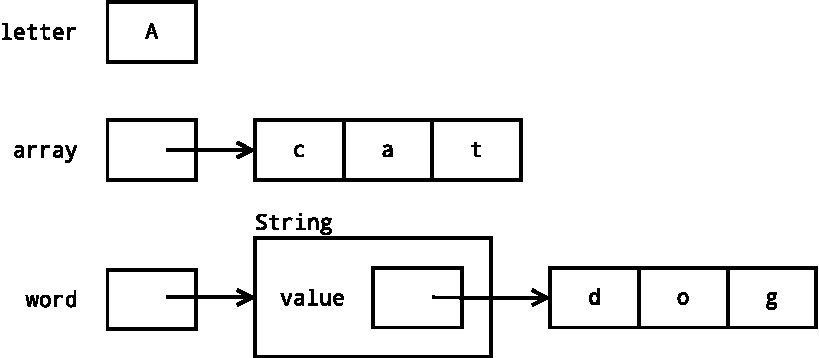
\includegraphics[width=\linewidth]{CS1/string1.pdf}
\null
\end{minipage}


\quest{15 min}


\Q How is the syntax of character literals and string literals different?

\begin{answer}
\end{answer}


\Q What is the index of \java{'d'} in the string above?
What is the index of \java{'g'}?
In general, what is the index of the last character of a string?

\begin{answer}
\end{answer}


\Q Based on the diagram, what does it mean for a class to encapsulate data?

\begin{answer}
\end{answer}


\Q Why can you use the \java{String} class in Java programs without having to import it first?

\begin{answer}
\end{answer}


\Q What is the value of a \java{char} variable?
What is the value of an array variable?
What is the value of a \java{String} variable?

\begin{answer}
\end{answer}


\Q Draw a memory diagram for the given code.
Each variable should be a name next to a box containing its value.

\vspace{1ex}
\begin{javalst}
String str;
str = "Hi!";

char let;
let = 'X';

int num;
num = -1;

double foo;
foo = num;

String hmm;
hmm = str;
\end{javalst}


\Q Recall that the == operator compares the \emph{value} of two variables.
What does it mean for two \java{char} variables to be ==?
What does it mean for two \java{String} variables to be ==?

\begin{answer}
\end{answer}


\Q How could you determine whether two character arrays have the same contents?
In other words, how does the \java{Arrays.equals} method work?

\begin{answer}
\end{answer}
